\documentclass[aspectratio=169,xcolor=dvipsnames]{beamer}
\usepackage[utf8]{inputenc}  % Required for umlauts
\usepackage[english]{babel}  % Language
%\usepackage[sfdefault]{roboto}  % Enable sans serif font roboto
%\usepackage{libertine}  % Enable this on Windows to allow for microtype
\usepackage[T1]{fontenc}  % Required for output of umlauts in PDF

\usepackage{mathtools,bbold}  % Required for formulas
\usepackage{siunitx}  % Give numbers units (with proper spacing)

\usepackage{caption}  % Customize caption aesthetics
\usepackage{tcolorbox}  % Fancy colored boxes
\usepackage{color}
\usepackage{xcolor}  % Highlighting
\usepackage{soul}

\usepackage{booktabs}  % Using pandas' LaTeX output
\usepackage{multirow}  % Enable fancy table structure
\usepackage{listings}  % Insert programming code
\usepackage{lstautogobble}  % Cleaner indentation in TeX file of code blocks within LaTeX blocks

\usepackage{graphicx}  % Required to insert images
\usepackage{subcaption}  % Enable sub-figure
\usepackage[space]{grffile}  % Insert images baring a filename which contains spaces
\usepackage{float}  % Allow to forcefully set the location of an object
% Include external standalone files such as Tikz graphics; requires `-shell-escape`
\usepackage{standalone}
\usepackage{tikz}  % Fancy drawing environment
\usepackage{pgfplots}  % Functions in Tikz
\usepackage[]{algorithm2e}  % Format fancy algorithms

\usepackage[tracking=true]{microtype} % Required to change character spacing

\usepackage[backend=biber,autocite=footnote,style=authoryear-icomp,sorting=none,doi=false,isbn=false,url=false,eprint=false]{biblatex}
\usepackage{csquotes}  % Ensure proper quotation of texts with babel and polyglossia with biblatex
\usepackage{hyperref}  % Insert clickable references

\usepackage{datetime}  % Flexible date specification

\usepackage{geometry}
\usepackage{scrextend}  % Allow arbitrary indentation

\usepackage{appendixnumberbeamer}  % Fancy page numbering excluding the appendix

% Compile notes into a separate file readable by pdfpc using a custom package which overwrite the `note` macro
\usepackage{pdfpcnotes}
% NOTE: Adding "noframenumbering" as argument to the first slide confuses `pdfpc`; see https://github.com/pdfpc/pdfpc/issues/367

\usetikzlibrary{patterns}
\usetikzlibrary{arrows}
\usetikzlibrary{matrix}
\usetikzlibrary{hobby}
\usetikzlibrary{shapes.misc}
\usetikzlibrary{shapes.callouts}
\pgfmathdeclarefunction{gauss}{2}{%
	\pgfmathparse{1/(#2*sqrt(2*pi))*exp(-((x-#1)^2)/(2*#2^2))}%
}

\addbibresource{literature.bib}
\renewcommand{\footnotesize}{\tiny}
%\renewcommand*{\bibfont}{\scriptsize}

\newcommand{\leadingzero}[1]{\ifnum#1<10 0\the#1\else\the#1\fi}
\newcommand{\todayddmmyyyy}{\leadingzero{\day}.\leadingzero{\month}.\the\year}
\newcommand{\mathcolorbox}[2]{\colorbox{#1}{$\displaystyle #2$}}

\DeclareMathOperator*{\argmin}{arg\,min}

\makeatletter
% Fix subfig in beamer style presentation
\let\@@magyar@captionfix\relax

% Insert [short title] for \section in ToC
\patchcmd{\beamer@section}{{#2}{\the\c@page}}{{#1}{\the\c@page}}{}{}
% Insert [short title] for \section in Navigation
\patchcmd{\beamer@section}{{\the\c@section}{\secname}}{{\the\c@section}{#1}}{}{}
% Insert [short title] for \subsection in ToC
\patchcmd{\beamer@subsection}{{#2}{\the\c@page}}{{#1}{\the\c@page}}{}{}
% Insert [short title] for \subsection in Navigation
\patchcmd{\beamer@subsection}{{\the\c@subsection}{#2}}{{\the\c@subsection}{#1}}{}{}
\makeatother

\definecolor{dodgerblue}{rgb}{0.06, 0.44, 0.8}
\setbeamercolor{tableofcontents}{fg=dodgerblue}
\setbeamercolor{section in toc}{fg=black}
\setbeamercolor{subsection in toc}{fg=black}
\setbeamercolor{block title}{fg=black}
\setbeamercolor{qed symbol}{fg=black}
\setbeamercolor{enumerate item}{fg=black}
\setbeamercolor{itemize item}{fg=black}
\setbeamercolor{itemize subitem}{fg=black}
\setbeamercolor{title}{fg=dodgerblue}
\setbeamerfont{title}{size=\LARGE}
\setbeamertemplate{title page}{%
	\vbox{}
	\begin{centering}
		\begin{beamercolorbox}[sep=8pt,center]{title}
			\usebeamerfont{title}\inserttitle\par%
			\ifx\insertsubtitle\@empty%
			\else%
				\vspace{0.25em}
				{\usebeamerfont{subtitle}\usebeamercolor[fg]{subtitle}\insertsubtitle\par}%
			\fi%
		\end{beamercolorbox}%
		\vspace{1em}\par
		\begin{beamercolorbox}[sep=8pt,center]{author}
			\usebeamerfont{author}\insertauthor%
		\end{beamercolorbox}
		\begin{beamercolorbox}[sep=8pt,center]{institute}
			\usebeamerfont{institute}\insertinstitute%
		\end{beamercolorbox}
		\begin{beamercolorbox}[sep=8pt,center]{date}
			\usebeamerfont{date}\insertdate%
		\end{beamercolorbox}%\vskip0.5em
	\end{centering}
}
\setbeamercolor{frametitle}{fg=dodgerblue}
\setbeamerfont{frametitle}{size=\LARGE}
\setbeamerfont{framesubtitle}{size=\small}
\setbeamertemplate{frametitle}{%
	\nointerlineskip%
	\hspace*{0.45em}
	% Other decent options are: `center`
	\begin{beamercolorbox}[ht=4em,sep=1em,wd=\paperwidth]{frametitle}
		\usebeamerfont{framesubtitle}
		\hspace{-0.3em}\strut\insertframetitle\strut%
		\\
		\usebeamerfont{frametitle}
		\strut\insertframesubtitle\strut%
	\end{beamercolorbox}
}
\setbeamercolor{footline}{fg=gray}
\setbeamercolor{date in head/foot}{fg=gray}
\setbeamercolor{author in head/foot}{fg=gray}
\setbeamercolor{section in head/foot}{fg=gray}
\setbeamerfont{footline}{size=\tiny}
\setbeamertemplate{footline}[text line]{%
	\leavevmode%
	\hspace*{-3.2em}
	\hbox{%
		\begin{beamercolorbox}[wd=.33\paperwidth,ht=1em,dp=0.5em,left]{date in head/foot}%
			\hspace{1.5em}
			\usebeamerfont{date in head/foot}\insertshortdate
		\end{beamercolorbox}%
		\begin{beamercolorbox}[wd=.33\paperwidth,ht=1em,dp=0.5em,center]{author in head/foot}%
			\usebeamerfont{author in head/foot}\insertshortauthor
		\end{beamercolorbox}%
		\begin{beamercolorbox}[wd=.33\paperwidth,ht=1em,dp=0.5em,right]{section in head/foot}%
			\usebeamerfont{date in head/foot}
			\insertframenumber{} %/ \inserttotalframenumber\hspace*{1em}  % NOTE, excessive for a 12 min. talk
			\hspace{1.5em}
		\end{beamercolorbox}
	}
}
\setbeamertemplate{navigation symbols}{}
\setbeamertemplate{itemize item}{$\bullet$}
\setbeamertemplate{itemize subitem}{$\circ$}
\captionsetup{font=scriptsize,labelfont={bf,scriptsize}}

% Customize code blocks
\definecolor{dodgerblue}{rgb}{0.06, 0.44, 0.8}
\definecolor{dodgerred}{rgb}{0.93, 0.24, 0.26}
\lstset{basicstyle=\fontsize{9}{11}\selectfont\ttfamily,
	breaklines=true,
	showstringspaces=false,
	commentstyle=\color{dodgerred},
	keywordstyle=\color{dodgerblue},
	frame=none,
	frameround=ffff,
	autogobble=true
}
\lstset{language=Python,
	rulecolor=\color{black},
	tabsize=2,
}

\title{NIFTy: The Why and How of Building AD from Scratch}
\subtitle{}
\author[Gordian Edenhofer]{%
	{\href{mailto:gordian.edenhofer@gmail.com}{Gordian Edenhofer}}\inst{1,2,3}
}
\institute[LMU]{%
	\inst{1}Max Planck Institute for Astrophysics, Garching, DE \\
	\inst{2}Faculty of Physics, LMU, Munich, DE \\
	\inst{3}Center for Astrophysics $\vert$ Harvard \& Smithsonian, Cambridge, MA, USA \\
}
\date[EnzymeCon]{Enzyme Conference 2023, \formatdate{23}{02}{2023}}
\subject{}

\begin{document}

% NOTES
% * Introduce myself!!!
% * Do NOT talk about TOC for a 12 min. talk

\pagenumbering{arabic}

\begin{frame}[plain]
	\titlepage%
	\note{%
		* From astrometric and photometric data to 3D dust
	}
\end{frame}

% Submitted Abstract
%
% Automatic Differentiation (AD) is the backbone of applied second order
% minimization schemes and used extensively for solving statistical inference
% problems. Both often require forward and reverse mode differentiation for
% efficiency. However, early AD frameworks did not support both. In 2013 this
% sparked the development of NIFTy, a Bayesian inference library with a
% (specialized) second order minimization scheme and a custom-built AD engine on
% top of NumPy. In this talk we introduce how NIFTy realizes AD via
% linearization- and transposition-rules. Furthermore, we discuss how using AD
% for second order minimization affects the choice of rematerialization
% strategies. Attendees will learn core concepts for building their own simple
% AD framework and why linearizations and transpositions are highly desirable
% for efficient second order minimization.

\section{AD in Astrophysical Imaging}  % Background
\frame[plain,noframenumbering]{\vfill\centering\tableofcontents[sectionstyle=show/shaded,subsectionstyle=show/hide]\vfill}

\subsection{What}  % Introduction, Background
{
\setbeamercolor{background canvas}{bg=black}
\begin{frame}[plain,noframenumbering]
	\begin{tikzpicture}[overlay, remember picture, every text node part/.style={align=center}]
		\node[anchor=north west,xshift=-0.15cm,yshift=-0.25cm] at (current page.north west)
		{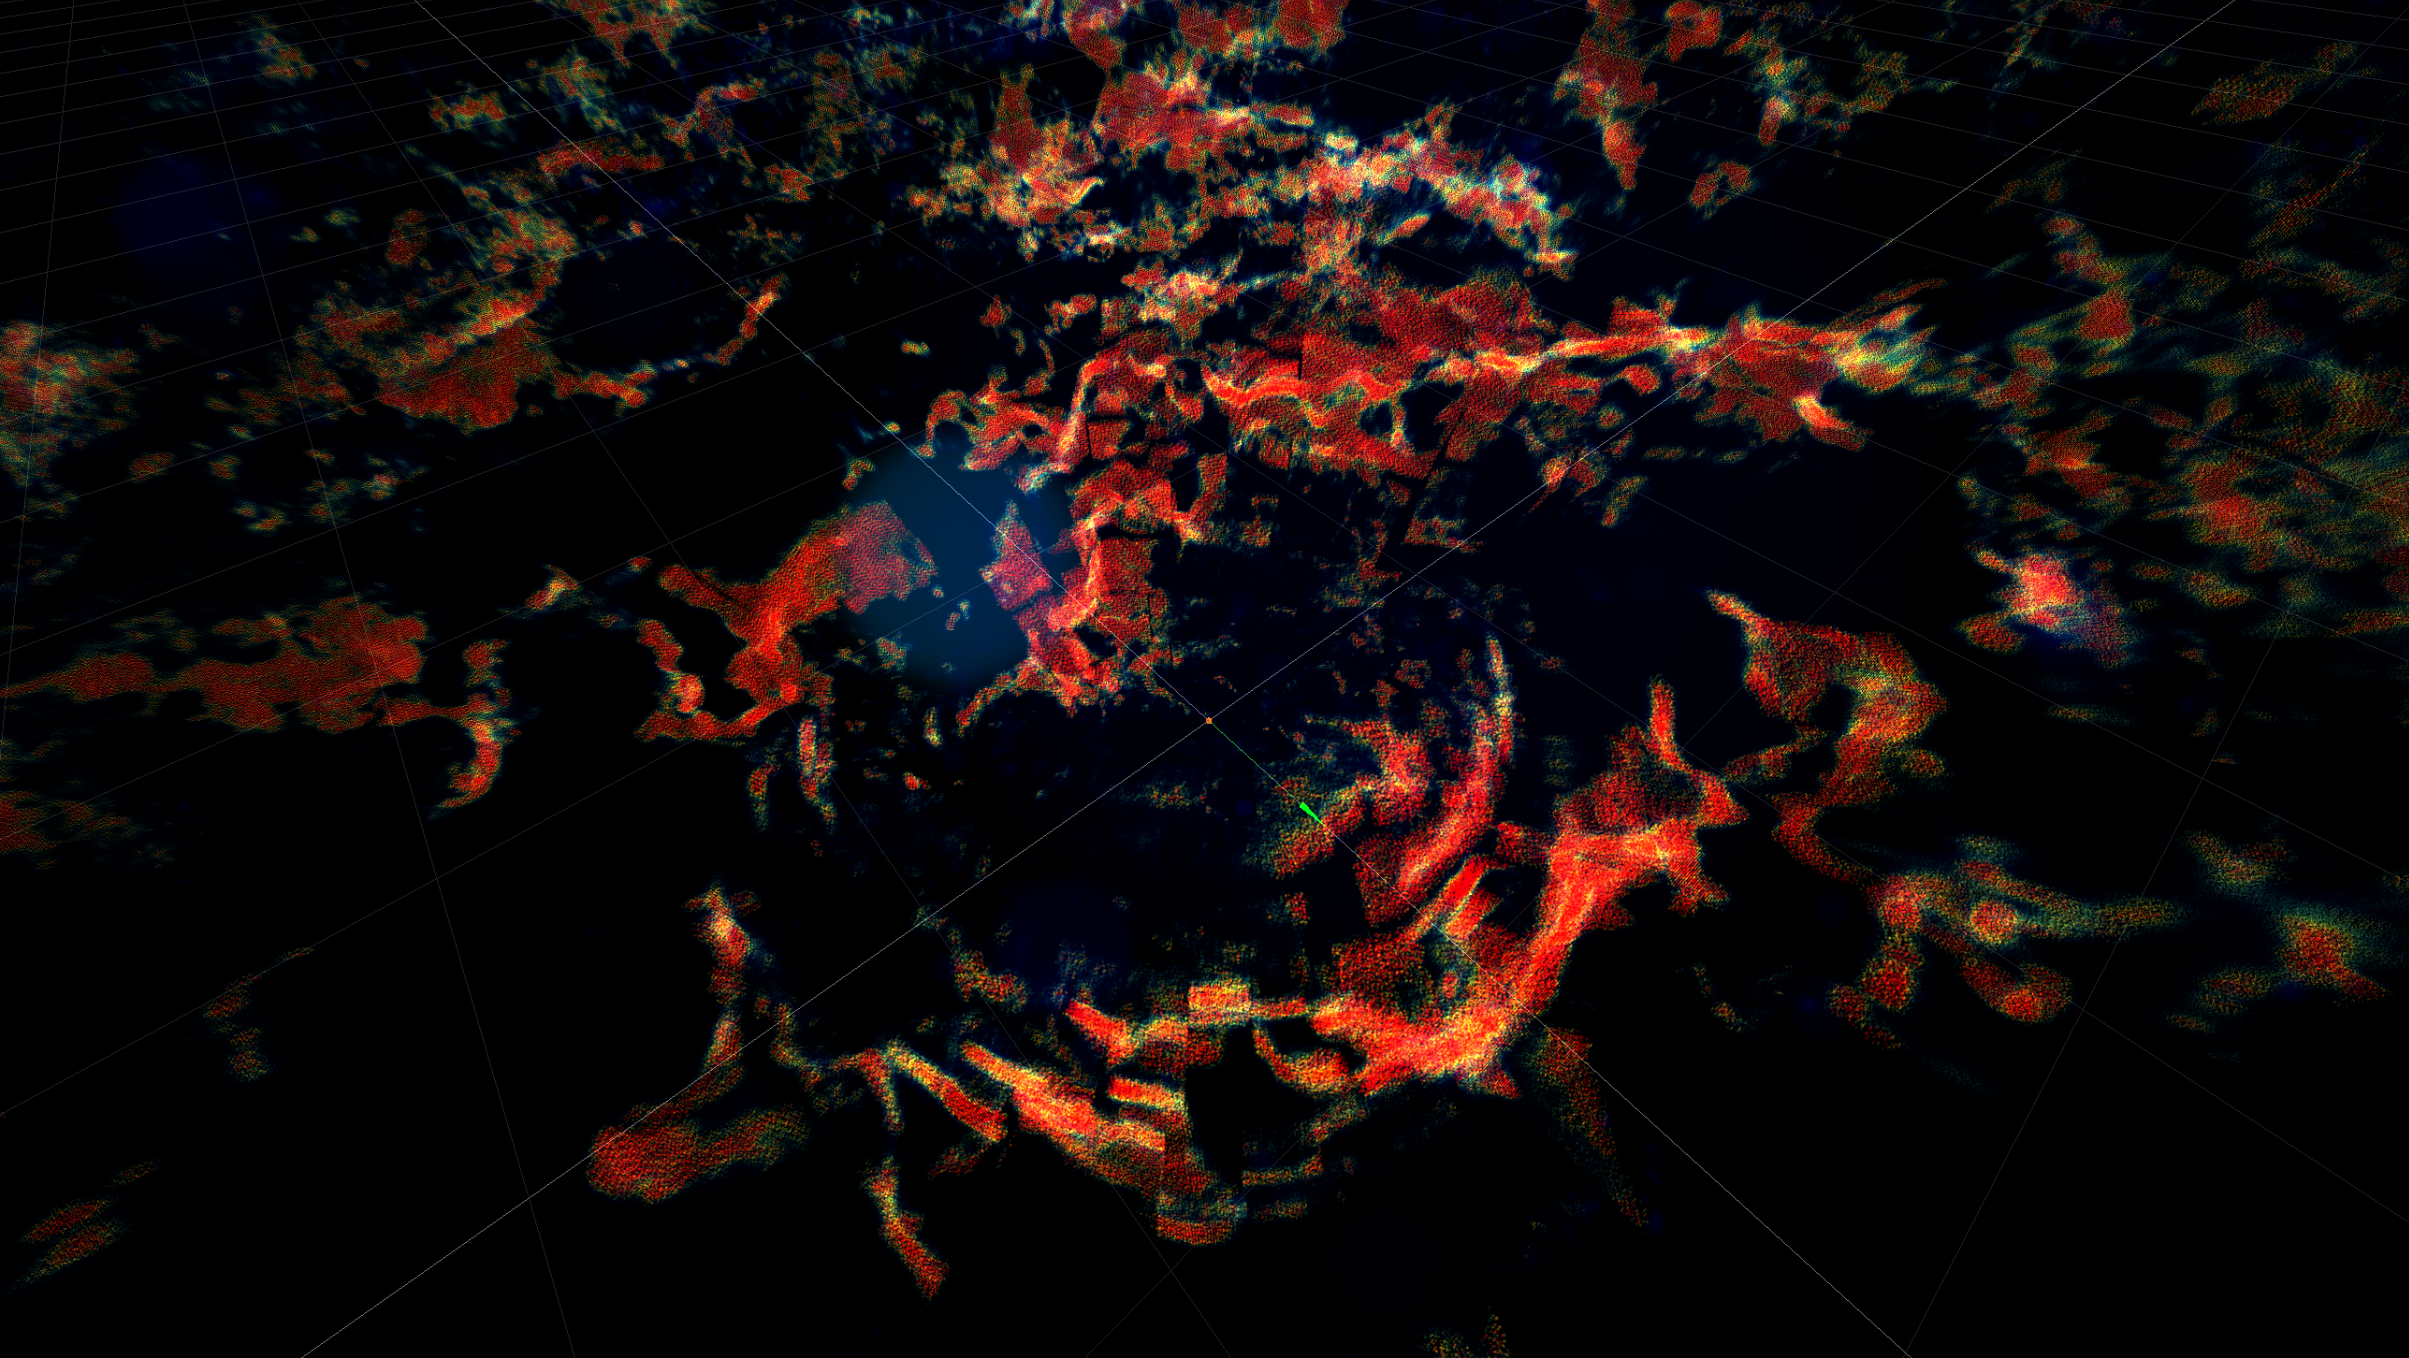
\includegraphics[width=1.145\textwidth,keepaspectratio]{{res/galactic_dust_off_axis_perspective}}};
	\end{tikzpicture}

	\note{* What I really want to do is 3D dust mapping}
	\note{* Meaning: statistical inference on lots of data with complicated model}
	\note{* Our approach to do so is by solving big optimization problem}
	\note{* Optimizations get faster if one uses derivates}
\end{frame}
}

\begin{frame}
	\frametitle{\insertsection}
	\framesubtitle{\insertsubsection}

	\begin{itemize}
		\item Statistical inference on $10\mathrm{M}+$ parameters can be rephrased to optimizing cost function of data $d$ and parameters $p$ (w.l.o.g.)
		\begin{align*}
			H(p) &= \ell(d, p) + p^\dagger p
			\\ &= \tilde{\ell}(d, f(p)) + p^\dagger p
		\end{align*}
		\pause
		\item From theory: Hessian $\partial^\dagger \partial H \approx J_{f}^\dagger \widehat{\tilde{L}} J_{f} + 1$ with $J_{f}$ the Jacobian of $f$ and some $\widehat{\tilde{L}'}$
		\pause
		\item Functional form of cost function $\rightarrow$ \colorbox{yellow}{easily accessible H'' $\rightarrow$ $2^\text{nd}$ order minimization}
	\end{itemize}

	\note{* So far the problem seems pretty generic, but I promise you it is not}
	\note{* 10M data points that can not simply be batched like in ML but need to be processed jointly}
	\note{* split of cost function is important}
	\note{* having to use full data + easily accessible Hessian approx. screams for second order AD}
\end{frame}

\subsection{Problems}  % Problem, Goal
\begin{frame}
	\frametitle{\insertsection}
	\framesubtitle{\insertsubsection}

	\begin{itemize}
		\item $2^\text{nd}$ order minimization $\rightarrow$ many ($\approx10^4$) calls to $\partial^\dagger \partial H$ few ($\approx10^3$) to $\partial H$
		\begin{enumerate}
			\item Get gradient
			\item Apply inverse Hessian to gradient $\rightarrow$ needs many calls to $\partial^\dagger \partial H$
			\item Take step \& repeat
		\end{enumerate}
		\pause
		\item (Most) AD tools focus on fast Jacobian-Vector-Product (JVP) or Vector-Jacobian-Poroduct (VJP)
		\begin{itemize}
			\item JVP reevaluates non-linearities
			\item VJP and JVP often do not share constants
			\item Unsuitable for $\partial^\dagger \partial H$
		\end{itemize}
	\end{itemize}

	\pause
	\begin{center}
		Numerical Information Field Theory = \colorbox{yellow}{DIY AD to make $\partial^\dagger \partial H  \approx J_{f}^\dagger \widehat{\tilde{L}} J_{f} + 1$ fast}
		\\ + (lots of statistics)
	\end{center}

	\note{* NIFTy custom AD for fast Hessian application}
	\note{* rest of the talk will focus on how to AD efficiently for our kind of problems}
	\note{* as a bonus you will learn how to build your own AD}
	% \footcitetext{Selig2013,Steiniger2019}
\end{frame}

\section{Linearizations on top of NumPy}  % Methodology
\frame[plain,noframenumbering]{\vfill\centering\tableofcontents[sectionstyle=show/shaded,subsectionstyle=show/hide]\vfill}

\subsection{Example}
\begin{frame}
	\frametitle{\insertsection}
	\framesubtitle{\insertsubsection}

	\begin{align*}
		f : \mathbb{R}^{n} &\rightarrow \mathbb{R}^k
		\\ p &\mapsto
		f(p) =
		\underbracket{\text{weighted\_reduction}}_{\text{implicit $k \times n$ matrix}}
		\circ
		\exp
		\circ
		\begin{bmatrix}
			p_{1} \\
			\vdots \\
			p_{n}
		\end{bmatrix}
	\end{align*}

	\pause
	\vspace{1em}
	\begin{center}
		$\partial^\dagger \partial H\approx J_{f}^\dagger \widehat{\tilde{L}} J_{f} + 1$ efficient iff $J_f \text{ and } J^\dagger_f$ efficient iff $J_f \text{ and } J^\dagger_f$ \colorbox{yellow}{fast} (skip non-linearities), \colorbox{yellow}{implicit} (no actual matrix) and \colorbox{yellow}{customizable} when necessary
		\vspace{0.5em}
		\\ here: no $\exp$ and always compute weighted reduction on the fly
	\end{center}

	\note{* constraints are essential; exp about seven times slower than mul}
	\note{* even current state-of-the-art AD models fail to fulfill them}
	\note{* complain about JAX}
\end{frame}

\subsection{Idea}
\begin{frame}
	\frametitle{\insertsection}
	\framesubtitle{\insertsubsection}

	Core concept: \colorbox{yellow}{Linearization}

	\pause
	\vspace{1em}
	Think of linearization $\leftrightarrow$ Jacobian as a function of two variables
	\begin{itemize}
		\item Primals $p$ for the location at which we linearize the function and
		\item Tangents $t$ to which we apply the linearization at $p$
	\end{itemize}
	\pause
	Linearization of operator $\mathrm{op}$ at $p$ is an (implicit) matrix $J_{\mathrm{op},p}$, Jacobian at $p$ applied to $t$ is an (implicit) matrix-vector product $J_{\mathrm{op},p} \cdot t$

	\pause
	\vspace{1em}
	We want linearization of $f$ for efficient $\partial^\dagger \partial H$

	\note{* Note the dependency on the position!}
	\note{* NIFTy is like reverse mode AD but for forward mode and reverse mode combined (no dual numbers)}
	\note{* non-linearities are made much cheaper here; imagine e.g. and exp in the forward model}
\end{frame}

\subsection{Idea}
\begin{frame}
	\frametitle{\insertsection}
	\framesubtitle{\insertsubsection}

	Overload operations $\mathrm{op}$ in $f$ with a dispatching rule to yield its linearization as well as its transpose and chain them together using the chain rule

	\begin{align*}
		\mathrm{op}: p &\mapsto \mathrm{op}(p)
		\\
		\downarrow
		\\
		\mathrm{op}: \mathrm{pl} &\mapsto
		\begin{cases}
			\mathrm{op}(\mathrm{pl}) & \text{if $\mathrm{pl}$ is of type numerics}
			\\ \text{Linearization}
				\begin{pmatrix}
					\mathrm{op}(\mathrm{pl})
					\\ J_{\mathrm{op},\mathrm{pl}_p} \cdot \mathrm{pl}
					\\ \mathrm{pl}^\dagger \cdot J_{\mathrm{op},\mathrm{pl}_p}^\dagger
				\end{pmatrix}
				& \text{if $\mathrm{pl}$ is of type linearization}
		\end{cases}
	\end{align*}
\end{frame}

\begin{frame}
	\frametitle{\insertsection}
	\framesubtitle{\insertsubsection}

	\begin{equation*}
		f(p) =
		\text{weighted\_reduction}
		\circ
		\exp
		\circ
		\begin{bmatrix}
			p_{1} \\
			\vdots \\
			p_{n}
		\end{bmatrix}
	\end{equation*}

	\vspace{1em}
	$\exp$: point-wise operator $\rightarrow$ linearization is diagonal operator
	\\ weighted\textunderscore{}reduction: linear operator $\rightarrow$ linearization is operator itself

	\pause
	\vspace{2em}
	\begin{center}
		\colorbox{yellow}{
			$J_{f,p} = J_{\text{wr},\exp(p)} \cdot J_{\exp,p}$
			\hspace{2em}
			and
			\hspace{2em}
			$J_{f,p}^\dagger = J_{\exp,p}^\dagger \cdot J_{\text{wr},exp(p)}^\dagger$
		}
	\end{center}

	\note{* Linearization of exp is a diagonal operator}
	\note{* Note how J_wr depends on exp(x) not x}
	\note{* weighted reduction is linear and derivative is operator itself}
\end{frame}

\subsection{Linearizations}
\begin{frame}[fragile]
	\frametitle{\insertsection}
	\framesubtitle{\insertsubsection}

	\begin{lstlisting}[language=python,escapechar=!]
		class Linearization():
			def __init__(self, p, fwd=lambda t: t, bwd=lambda t: t):
				self.p = p  # new primals after applying the non-linearized !$J$!
				self._fwd, self._bwd = fwd, bwd  # !$J, J^\dagger$!

			def __call__(self, t):  # !$J \cdot t$! with tangents !$t$!
				return self._fwd(t)

			@property
			def T(self):  # !$J^\dagger$!
				return self.__class__(None, self._bwd, self._fwd)

			# optional: implement infix arithmetics
	\end{lstlisting}

	\note{* I promised showing how to build your own AD: so here we go}
	\note{* linearization needs to know position as to amend it}
	\note{* linearization needs to forward pass = J_f}
	\note{* linearization needs to backward pass = J_f^+}
\end{frame}

\begin{frame}[fragile]
	\frametitle{\insertsection}
	\framesubtitle{\insertsubsection}

	\begin{lstlisting}[language=python,escapechar=!]
		def exp(pl):
			if not isinstance(pl, Linearization):  # primals or linearization
				return np.exp(pl)  # new primals
			!\pause!
			y = exp(pl.p)  # new primals
			def fwd(t): return y * pl(t)  # !\colorbox{yellow}{chain rule: $J_{\exp,\mathrm{pl.p}} \cdot J_\mathrm{pl} \cdot t$}!
			def bwd(t): return pl.T(y * t)  # !\colorbox{yellow}{chain rule: $J^\dagger_\mathrm{pl} \cdot J^\dagger_{\exp,\mathrm{pl.p}} \cdot t$}!
			return Linearization(y, fwd, bwd)
	\end{lstlisting}

	\pause
	\begin{lstlisting}[language=python,escapechar=!]
		x0 = 1e-2 * np.arange(0, 9)
		ones = np.ones((9, ))
		y = exp(x0)
		j = exp(exp(Linearization(x0)))
		j.T(ones)
	\end{lstlisting}

	\note{* Note how the linearization and its adjoin is successively amended}
	\note{* Amending relies on closures}
	\note{* linearization differ from JVP/VJP in that they do not evaluate the original function}
	\note{* Forward and backward have no exp in them}
	\note{* Note, we reference `exp` back in Linearization call -> arbitrary order}
\end{frame}

\begin{frame}[fragile]
	\frametitle{\insertsection}
	\framesubtitle{\insertsubsection}

	\begin{lstlisting}[language=python,escapechar=!]
		def weighted_reduction(pl, n=32, n_cols=3):
			if not isinstance(pl, Linearization):  # primals or linearization
				p = pl.reshape(n_cols, -1)
				y, indices = np.zeros((n, )), np.arange(n) % p.shape[0]
				for i, idx in enumerate(indices):
					super_expensive_weights = np.ones(p.shape[1:])  # large weights
					y[i] = np.sum(p[idx] * super_expensive_weights)
				return y  # new primals !\pause!
			def fwd(x): return weighted_reduction(pl(x))  # !\colorbox{yellow}{ref. to self}!
			def bwd(x): ...
			return Linearization(weighted_reduction(pl.p), fwd, bwd)
	\end{lstlisting}

	\pause
	\begin{lstlisting}[language=python,escapechar=!]
		y2 = weighted_reduction(y)
		j = weighted_reduction(Linearization(y))
		j(y)
	\end{lstlisting}

	\note{* Forward pass in linearization is operator itself}
\end{frame}

\subsection{Linearizations for minimization objective}
\begin{frame}[fragile]
	\frametitle{\insertsection}
	\framesubtitle{\insertsubsection}

	\begin{lstlisting}[language=python,escapechar=!]
		def f(x):
			return weighted_reduction(exp(x))

		x0 = 1e-2 * np.arange(0, 9)
		f0 = f(x0)
		f_ones = np.ones(f0.shape)

		j = f(Linearization(x0))
		j(x0), j.T(f_ones)
	\end{lstlisting}

	\note{* let's get back to original demo of chained cost function}
	\note{* get linearizations by putting linearization into model}
\end{frame}

\begin{frame}[fragile]
	\frametitle{\insertsection}
	\framesubtitle{\insertsubsection}

	\begin{align*}
		H(p) = \tilde{\ell}(d, f(p)) + p^\dagger p \quad\quad \partial^\dagger \partial H \approx J_{f}^\dagger \widehat{\tilde{L}} J_{f} + 1
	\end{align*}

	\vspace{1em}
	\begin{lstlisting}[language=python,escapechar=!]
		def h(p):  # Cost function with Gaussian likelihood and unit noise
			return sum((d - f(p))**2) + sum(p**2)
		!\pause!
		def gradient(p):  # gradient at !$p$! is VJP at !$p$! applied to 1.
			return h(Linearization(p)).T(1.)
		!\pause!
		def hessian_at(p):  # approx. hessian at !$p$! acting on !$t$!
			j = f(Linearization(p))
			def h_at_p(t): return j.T(l_prime(j(t))) + t
			return h_at_p
	\end{lstlisting}

	\note{* congrats, you now understand the DIY AD in NIFTy}
\end{frame}

\begin{frame}
	\frametitle{\insertsection}
	\framesubtitle{\insertsubsection}

	\begin{itemize}
		\item Fast
		\begin{itemize}
			\item Skip non-linearities
			\item Fast if individual computations are fast
		\end{itemize}
		\pause
		\item Implicit: NIFTy thinks in terms of linearizations and wraps almost all of NumPy
		\pause
		\item Customizable Jacobians
		\begin{itemize}
			\item Jacobian of model is automatically derived via chain-rule
			\item Trivial to redefine Jacobian for model via above schema
			\item Convenience of python
		\end{itemize}
	\end{itemize}

	\note{* NIFTy is fast if model is dominated by computations and not python (think: pytorch)}
\end{frame}

\subsection{Checkpointing}
\begin{frame}
	\frametitle{\insertsection}
	\framesubtitle{\insertsubsection}

	Checkpointing a.k.a. rematerialization strategy = storing versus recomputing values required for AD

	\begin{itemize}
		\item Crucial as \#parameter and constants in astrophysical models can be huge
		\item Computation versus memory tradeoff impossible in general $\rightarrow$ needs user input
		\item $J_{f,x}$ and $J_{f,x}^\dagger$ can almost always share constants
	\end{itemize}

	\note{* Memory versus computation tradeoff}
	\note{* NIFTy's design incentivizes sharing memory between forward and backward}
	\note{* DIY in NIFTy}
	\note{* looking at you JAX for excessive memory allocation for transpositions}
\end{frame}

\begin{frame}[fragile]
	\frametitle{\insertsection}
	\framesubtitle{\insertsubsection}

	\vspace{-1em}
	\begin{lstlisting}[language=python,escapechar=!,basicstyle=\fontsize{8}{9}\selectfont\ttfamily]
		def weighted_reduction(pl, n=32, n_cols=3):
			if not isinstance(pl, Linearization):  # primals or linearization
				p = pl.reshape(n_cols, -1)
				y, indices = np.zeros((n, )), np.arange(n) % p.shape[0]
				for i, idx in enumerate(indices):
					super_expensive_weights = np.ones(p.shape[1:])  # large weights
					y[i] = np.sum(p[idx] * super_expensive_weights)
				return y  # new primals

			def fwd(x): return weighted_reduction(pl(x))  # new primals
			def bwd(x):  # !\colorbox{yellow}{implicit $J^\dagger_{\mathrm{wr},\mathrm{pl.p}}$ which re-computes all weights}!
				p_shp = pl.p.reshape(n_cols, -1).shape
				x_T, indices = np.zeros(p_shp), np.arange(n) % p_shp[0]
				for i, idx in enumerate(indices):
					super_expensive_weights = np.ones(p_shp[1:])
					x_T[idx] += x[i] * super_expensive_weights
				return pl.T(x_T.reshape(pl.p.shape))
			return Linearization(weighted_reduction(pl.p), fwd, bwd)
	\end{lstlisting}
\end{frame}

\section{Numerical Information Field Theory}  % Result
\frame[plain,noframenumbering]{\vfill\centering\tableofcontents[sectionstyle=show/shaded,subsectionstyle=show/hide]\vfill}

% \subsection{Linearizations in NIFTy}
% \begin{frame}
% 	\frametitle{\insertsection}
% 	\framesubtitle{\insertsubsection}

% 	NIFTy is designed for large statistical models with 10+M parameters
% 	\vspace{1em}
% 	Computational cost dominated Hessian calls
% 	\vspace{1em}
% 	Hessian calls dominated by few inherently expensive operations (often \texttt{FFT})
% 	\vspace{1em}
% 	Fast if individal computations are expensive and done efficiently outside of python
% \end{frame}

\subsection{NIFTy AD}
\begin{frame}[fragile]
	\frametitle{\insertsection}
	\framesubtitle{\insertsubsection}

	\begin{lstlisting}[language=python,escapechar=!]
		x = ...
		model = ift.LOSResponse(correlated_field.target, ...) \
			@ ift.exp \
			@ x

		x0 = ...
		j = model(ift.Linearization.make_var(x0))
	\end{lstlisting}

	\vspace{1em}
	\begin{center}
		Fast, implicit, and customizable linearizations with the convenience of python
	\end{center}

	\note{* NIFTy is made for astrophysical inference}
	\note{* NIFTy implements custom posterior approximation techniques}
	\note{* NIFTy implements cool modeling tools for representing smoothness, e.g. for dust clouds}
	\note{* make bottlenecks go brrr with C++}
	\note{* this is how we infer models with 10M+ parameters}
\end{frame}

\begin{frame}
	\frametitle{\insertsection}
	\framesubtitle{\insertsubsection}

	\begin{itemize}
		\item[] Linearizations are convenient concept for AD (especially for $2^\text{nd}$ order minimization)
		\begin{itemize}
			\item Never re-evaluates non-linearities
			\item By NIFTy design incentivizes sharing memory (and code) between $J$ and $J^\dagger$
		\vspace{2em}
		\end{itemize}
		\item[] Building your own AD is actually pretty simple
	\end{itemize}

\end{frame}

\end{document}
